\chapter{DAH Projects}
\label{sec:projects}
%
All the projects involve analysis of data taken by the LHCb experiment. For more information on LHCb you are refered to  {DOI:10.1007/JHEP06(2013)064).}. The data is presented to allow you to do this in a simplified way but the steps you will follow are similar to what is done in any real analysis
\begin{itemize}
\item Make simple checks of the data, for example making histograms and using these to estimate the position and width of peaks.
\item Perform fits to invariant mass distributions to determine the yield of particles.
\item Apply cuts to improve the signal to background or to select a specific region of space space.
\item Compare your results to theory expectations and previous studies.
\end{itemize}
The projects have been designed in to explore the data in different ways and to chose your own adventure. They all start from binary files which store around six different variables for different datasets collected by LHCb. The meaning of these variables may not be immediately clear to you at the start of the project and this is something you will need to think about. You should think  about what the advantages and disadvantages of storing binary information are. Some of the data files used in the project are rather large. Fitting large datasets without binning can be computationally challenging and you may consider a binned fit if appropriate.

We are assuming for the projects that all of you have a laptop and will on this remotely. If you need access to the CPLab computers on the desks in the DAH laboratories to perform the project you should contact the course organizers.

\section{Project F1: Make Accurate Measurements of $\Upsilon$  Masses}

\subsection{Goals of project}
%
You will use LHCb data on the invariant mass of $\Upsilon$ particle candidates collected in 2015. You will first make simple checks of the data and get first estimates of peak positions and widths.  Next you will use the maximum likelihood process to fit different mass model shapes to the data. From this you will determine the parameters of the mass model for the three signal peaks, and their errors. You will start with a very simple Gaussian mass model. You will then improve this and use a more sophisticated model.

The project has an open-ended aspect and are an opportunity where you can show your own initiative and demonstrate your experimental and computational skills. 

\subsection{Detailed project description}

The LHCb experiment at the Large Hadron Collider at CERN has recorded a sample of muon pairs with invariant masses in the range of 8.5 to 11 GeV/$c^2$. Three clear peaks are observed in this mass spectrum. These correspond to the production of Upsilon mesons, which are bound states of a $b$ and a anti-$b$ quark. These states are known as the $\Upsilon \rm (1S)$, $\Upsilon \rm (2S)$ and $\Upsilon \rm (3S)$ mesons where the $\Upsilon \rm (1S)$ meson is the ground state and the $\Upsilon \rm (2S)$  and $\Upsilon \rm (3S)$  states are radial excitations (for LHCb paper, see {DOI: 10.1007/JHEP06(2013)064).}

\begin{center}
    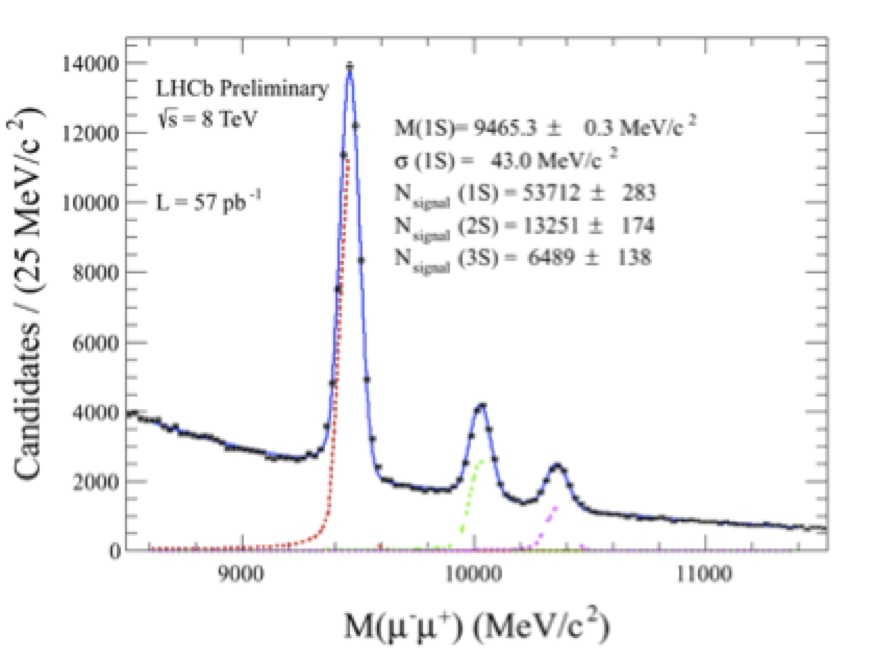
\includegraphics[width=9cm]{figs/mu-pair-mass}
\end{center}

Download the files ups-15.bin, ups-15-small.bin and mc.bin   from the DAH Dropbox, 
The first  two files contain the data recorded by LHCb in 2015 and a subset with a factor 5 less data. 
In addition, there is a file with simulated data (Monte Carlo).
The files are written in binary format and contain five observables for a large number of muon pairs
\begin{itemize}
\item  invariant mass of muon pair in   GeV/$c^2$;
\item transverse momentum $p_\perp$ of muon pair in GeV/$c$;
\item rapidity $\eta$ of muon pair;
\item  momentum $p$ of muon pair in GeV/$c$;
\item transverse momentum $pt$ of first muon in GeV/$c$;
\item transverse momentum $pt$ of second muon in GeV/$c$.
\end{itemize}

Write a python script that reads the data from this file, see below. 

\lstinputlisting{../scripts/project_F_a.py}
\vspace*{-0.5cm}

Start with the small ups-15-small.bin file. Plot histograms of all six variables, choosing a reasonable bin width. Always label plots correctly with title and axes and save these to a file. [Hint: The bin width should be chosen such that each of the three peaks is clearly resolved and represented by a sufficient number of bins for analysis.]

Next, make some estimates of the peak positions and widths using the histogram of invariant mass.  Determine the masses of the three particles by determining the bins with the highest number of entries in the peak regions. Divide the histogram into three peak regions and write a local peak finding method for this part.
What are the mass differences between the $\Upsilon \rm (2S)$ and $\Upsilon \rm (3S)$ states with respect to the $\Upsilon \rm (1S)$ meson. By inspecting visually the muon-pair mass spectrum, determine the Full Width Half Maximum (FWHM) of the $\Upsilon \rm (1S)$ mass peak. Assuming a Gaussian signal shape estimate the mass resolution $\sigma$ from the FWHM. %of the $\Upsilon \rm (1S)$  peak.

In the muon-pair mass spectrum define a signal region of width $\pm 150\; {\rm MeV}/c^2$ around the $\Upsilon \rm (1S)$  peak position and determine the number of events $N$ in this region.
Define an upper and lower sideband region where there are only background events. These sidebands should each be half as wide as the signal region and located at masses equidistant from the $\Upsilon \rm (1S)$  peak position. Assuming that the background is falling linearly with the muon-pair mass, determine the number of background events $B$ in the signal region (below the $\Upsilon \rm (1S)$  mass peak). Perform either a linear least squares fit in the sideband regions or use the sideband subtraction method for this. Determine the number of signal events $S$ in the signal region.

\begin{enumerate}
\item Consider first the $\Upsilon \rm (1S)$ particle, which is the particle with the lowest mass, i.e. the left most  peak in the plot. Construct a composite probability density function (PDF) for the invariant mass of the muon pairs, which contains two components:
\begin{itemize}
\item A Gaussian shape to fit the  $\Upsilon \rm (1S)$ mass peak;
\item A shallow falling exponential to fit the background shape of the mass spectrum underneath and around the peak.
\end{itemize}

\item Use this PDF in a Maximum Likelihood fit to determine the parameters of the PDF. Note that it is essential that the composite PDF remains normalised to 1 over the range of the fit.

Determine the $\Upsilon \rm (1S)$  meson mass and yield, and all other parameters, and their and errors.

You should be able to obtain the parameter errors directly from the minimization engine of your choice (scipy.optimize.minimise, scipy.optimise.curve\_fit, lmfit, see \url{https://lmfit.github.io/lmfit-py/} or Minuit). Depending on your choice you will be able to chose different minimising methods.
It would be good to show that you understand these by obtaining them yourself from the parameters of the Gaussian signal fit - this is described in the data handling lectures.

Plot the fitted signal shape on top of the data.

\item Now consider the entire mass range, and perform a simultaneous fit for all three Upsilon peaks, and the underlying background. Again you should always report the parameter values, and their errors. Plot the fitted signal shape on top of the data.

\item The results so far probably look "quite good" by eye.  i.e. the signal shape plotted on top of the data probably looks like it fits quite well.  However this can be misleading when performing a precision measurement.  You should make a plot of what are called the "residuals". A residual is the difference between the data in the binned histogram and the best-fit mass model value for the centre of that bin. Describe what you see.

\item There are several ways to enhance the scope of the project. For example, if the single Gaussian mass model does not fit the data perfectly, one can try other mass models, i.e. by using a signal PDF that goes beyond a single Gaussian function.  Examples are:
\begin{itemize}
\item A PDF comprising a function which is the sum of two Gaussian functions (i.e. one narrow and one wide Gaussian function to fit a single Upsilon mass peak)
\item A Crystal Ball function, which incorporates a non-Gaussian tail at the lower end of the mass peak. The functional shape is described elsewhere, e.g. see: \url{http://en.wikipedia.org/wiki/Crystal_Ball_function}. 
\end{itemize}
Implement one or both of these functions in your PDF. 
First fit this PDF using the simulated Monte Carlo data. This allows you to see better
how the additional parameters should improve the description of the tails of the signal peak.
Then fit the PDF to the LHCb data and see how much better they are at describing the data.
Consider fixing some of the shape parameters from the fit to the Monte Carlo sample.

\item Make 2-dimensional plots of the additional observables vs the invariant mass of the muon pair.
Find out if you can improve the purity of your signal sample using the information in the file.
The purity is defined as the ratio of signal events over all events in a region.

\item As on open ended activity, you will see in the paper that the analysis is also done by dividing the data up into bins of transverse momentum ($pt$) and pseudorapidity ($\eta$). You can explore doing this analysis yourself and try to make the cross-section in bins of pT or eta. In particular taking ratios of yields will allow you to cancel the detector acceptance.
  
\item Read the publication and see what is said about systematic errors.  Make a reasonable attempt at determining some systematic errors on the masses.


\end{enumerate}

\subsection{Project planning}

The project descriptions are generally significantly less detailed than what was made available for the checkpoints. Any material covered during checkpoints including python code examples are assumed to be known.  Only essential and new information is provided and you are expected to take care of the details. Python code snippets are provided where necessary, but you will have to understand yourself what they do. It is recommend that you google for information about your project on the web, including data sheets of components and python libraries, if applicable. Python scripts should be well structured, either using functions or classes.

The timeline will vary between different projects, but in general, it is recommended that you plan your work as follows:
\begin{itemize}
\item	weeks 7, 8 \& 9: 	Building your gadget and/or writing code for project;
\item	week 9, 10: 	Analysis of data or equivalent, prepare supplementary material;
\item	week 10, 11:	Finish writing of project report and prepare submission.
\end{itemize}
Note that you are advised to start writing your report as the project progresses. 

For guidance on report writing, how the projects will be assessed, plagiarism and the submission deadline, please consult the DAH course booklet and the DAH grade descriptors, available on Learn.

 
 
 
\newpage
\section{Project F2: Make Accurate Measurements of Open charm meson Masses}
%
You will use LHCb data to study the mass of open charm mesons. You will first make simple checks of the data and get first estimates of peak positions and widths. You will use the maximum likelihood process to fit different mass model shapes to the data. From this you will determine the parameters of the mass model for the signal peaks, and their errors. You will start with a very simple Gaussian mass model. You will then improve this and use a more sophisticated model. 

The projects have an open-ended aspect and are an opportunity where you can show your own initiative and demonstrate your experimental and computational skills.



\subsection{Detailed project description}
 
In this project you will explore another LHCb dataset collected in 2011 where a pair of
oppositely charged kaons and a pion have been combined. Two clear
peaks are observed in this mass spectrum corresponding to the $D_s^+$ (quark content $c\overline{s}$)
and $D^+$ (quark content $c\overline{d}$) mesons (charge conjugation is implied), see figure below % (Fig.~\ref{fig:dmass}). 
For more information see: {DOI:10.1007/JHEP06(2013)065}. 
%
%\begin{figure}[htb!]
\begin{center}
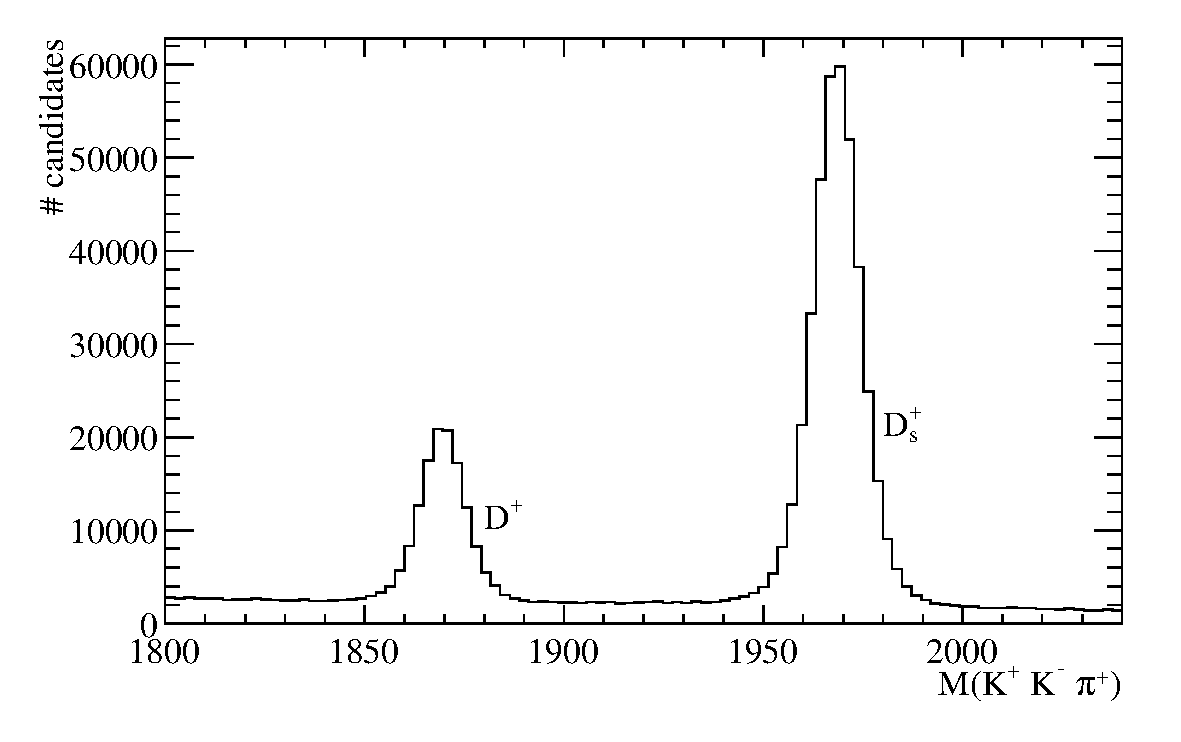
\includegraphics[width=0.75\textwidth]{figs/KKpi.pdf}\\
%\caption
{\small $K^{+}K^{-}\pi^{+}$ invariant mass distribution.}
%\label{fig:dmass}
\end{center}
%\end{figure}
%

Download the files kkp.bin and kkpp.bin files  from the DAH Dropbox, 
These files contain the data recorded by LHCb in 2011 for $D_{(s)}^+$ and $D^0$ decays respectively. Focus on the $D_{(s)}^+$ data file (kkp.bin):
The files are written in binary format and contain seven observables
\begin{itemize}
\item  invariant mass of $K^{+}K^{-}\pi^{+}$  candidate  in  MeV/$c^2$;
\item  invariant mass of kaon pair in   MeV/$c^2$;
\item transverse momentum of  $K^{+}K^{-}\pi^{+}$  candidate  in GeV/$c$;
\item rapidity $\eta$ of $K^{+}K^{-}\pi^{+}$  candidate;
\item minimum tranverse momentum of the three tracks in the $K^{+}K^{-}\pi^{+}$  candidate;
\item electric charge of the candidate;
\item Polarity of the LHCb magnetic field.
\end{itemize}

Write a python script that reads the data from this file, see below. 
\lstinputlisting{../scripts/project_F_b.py}
%\vspace*{-0.5cm}

\begin{enumerate}

\item Plot histograms of all variables, choosing a reasonable bin width. Always label plots correctly with title and axes and save these to a file. [Hint: The bin width should be chosen such that each of the three peaks is clearly resolved and represented by a sufficient number of bins for analysis.]

\item Next, make some estimates of the peak positions and widths using the histogram of invariant mass.  Determine the masses of the two particles by determining the bins with the highest number of entries in the peak regions. Divide the histogram into two peak regions and write a local peak finding method for this part. What is the mass differences between the $D_s^+$ and $D^+$ state ? By inspecting visually the mass spectrum, determine the Full Width Half Maximum (FWHM) of the $D_s^+$ mass peak. Assuming a Gaussian signal shape estimate the mass resolution $\sigma$ from the FWHM.

\item In the  $K^{+}K^{-}\pi^{+}$  mass spectrum define a signal region of width $\pm 25\; {\rm MeV}/c^2$ around the $D_s^+$  peak position and determine the number of events $N$ in this region.
Define an upper and lower sideband region where there are only background events. These sidebands should each be half as wide as the signal region and located at masses equidistant from the $D_s^+$  peak position. Assuming that the background is falling linearly with the mass, determine the number of background events $B$ in the signal region (below the $D_s^+$ peak). Perform either a linear least squares fit in the sideband regions or use the sideband subtraction method for this. Determine the number of signal events $S$ in the signal region.

\item Consider first the $D_s^+$ peak which is the particle with the higher
mass, i.e. the right most peak in the plot. Construct a composite probability density
function (PDF) for the invariant mass of the muon pairs, which
contains two components : 
\begin{itemize}
\item A Gaussian shape to fit the  $D_s^+$ mass peak;
\item A shallow falling exponential to fit the background shape of the mass spectrum underneath and around the peak.
\end{itemize}

\item	Use this PDF in a Maximum Likelihood fit to determine the parameters of the PDF. Note hat it is essential that the composite PDF remains normalised to 1 over the range of the fit.

Determine the $D^+$  meson mass and yield, and all other parameters, and their and errors.

You should be able to obtain the parameter errors directly from the minimization engine of your choice (scipy.optimize.minimise, scipy.optimise.curve\_fit, lmfit, see \url{https://lmfit.github.io/lmfit-py/} or Minuit). Depending on your choice you will be able to chose different minimising methods.
It would be good to show that you understand these by obtaining them yourself from the parameters of the Gaussian signal fit - this is described in the data handling lectures.

Plot the fitted signal shape on top of the data.

\item Now consider the entire mass range, and perform a simultaneous fit for both
peaks, and the underlying background. Again you should always report the parameter
values, and their errors. Plot the fitted signal shape on top of the data.
\item The results so far probably look quite good by eye. i.e. the signal shape plotted on
top of the data probably looks like it fits quite well. However this can be misleading
when performing a precision measurement. You should make a plot of what are called
the residuals. A residual is the difference between the data in the binned histogram
and the best-fit mass model value for the centre of that bin. Describe what you see.
\item There are several ways to enhance the scope of the project.

\begin{itemize} 
\item For example, if the single
Gaussian mass model does not fit the data perfectly, one can try other mass models,
i.e. by using a signal PDF that goes beyond a single Gaussian
function. One example: is a PDF comprising a function which is the sum of two Gaussian functions (i.e. one
narrow and one wide Gaussian function to fit a single $D_{(s)}$ meson
peak. Alternatively try a Crystal Ball function, which incorporates a non-Gaussian tail at the lower end of
the mass peak. The functional shape is described elsewhere, e.g. see:
\begin{verbatim}
https://en.wikipedia.org/wiki/Crystal_Ball_function 
\end{verbatim} 
You could implement each of these functions in your PDF and see how much better
they are at describing the data.
\item Read the publication and see what is said about systematic errors. Make a reasonable
attempt at determining some systematic errors on the masses.
\item Compare your results to the PDG and previous measurements.
\item Study how the mass and the width of the peak (the resolution)
  depends on the transverse momentum (pt) and rapidity (eta).
\item In the data file you are provided with the charge of the D meson and the magnetic field polarity. Divide up the data into different categories of charge and polarity and remake the fits. What can you learn from these studies ?
\item Investigate whethe the mass of kaon pair and the minimum tranverse momentum of the
 daughter particles can be used to improve the purity of the sample.
\item An additional file has been provided of candidates for the decay $D^0 \rightarrow K^+ K^- \pi^+ \pi^-$. Use this file to estimate the mass splitting between the charged and neutral D mesons and compare to the PDG. The variables in this file are the candidate mass, the mass of the kaon pair, pt, eta, ptmin and field polarity.
\end{itemize}



\end{enumerate}

\subsection{Project planning}

The project descriptions are generally significantly less detailed than what was made available for the checkpoints. Any material covered during checkpoints including python code examples are assumed to be known.  Only essential and new information is provided and you are expected to take care of the details. Python code snippets are provided where necessary, but you will have to understand yourself what they do. It is recommend that you google for information about your project on the web, including data sheets of components and python libraries, if applicable. Python scripts should be well structured, either using functions or classes.

The timeline will vary between different projects, but in general, it is recommended that you plan your work as follows:
\begin{itemize}
\item	weeks 7, 8 \& 9: 	Building your gadget and/or writing code for project;
\item	week 9, 10: 	Analysis of data or equivalent, prepare supplementary material;
\item	week 10, 11:	Finish writing of project report and prepare submission.
\end{itemize}
Note that you are advised to start writing your report as the project progresses. 

For guidance on report writing, how the projects will be assessed, plagiarism and the submission deadline, please consult the DAH course booklet and the DAH grade descriptors, available on Learn.

 

\newpage
\section{Project F3: Production of $J/\psi$ mesons}

\subsection{Goals of project}

You will use LHCb data on the the production and properties of $J/\psi$ mesons. You will first make simple checks of the data and get first estimates of peak positions and widths. You will use the maximum likelihood process to fit different mass model shapes to the data. From this you will determine the parameters of the mass model for the signal peak, and their errors. You will start with a very simple Gaussian mass model. You will then improve this and use a more sophisticated model.

The project has an open-ended aspect and are an opportunity where you can show your own initiative and demonstrate your experimental and computational skills. 




\subsection{Detailed project description}
 
In this project you will explore an LHCb dataset where the decay a pair of oppositely charged muons originating from the decay of a $J/\psi$ meson ( a $c\overline{c}$ state) is reconstructed. The $J/\psi$ can be produced in different procsses but in this case selection requirements have been applied that select $J/\psi$ produced in decays of the $b$-quark. For more information see  {DOI:10.1007/JHEP1Dro(2015)172}. The data you are using comes from later LHCb running during 2016. A downscale of 10 has been applied but the dataset is still large. 

%
%\Begin{figure}[htb!]
\begin{center}
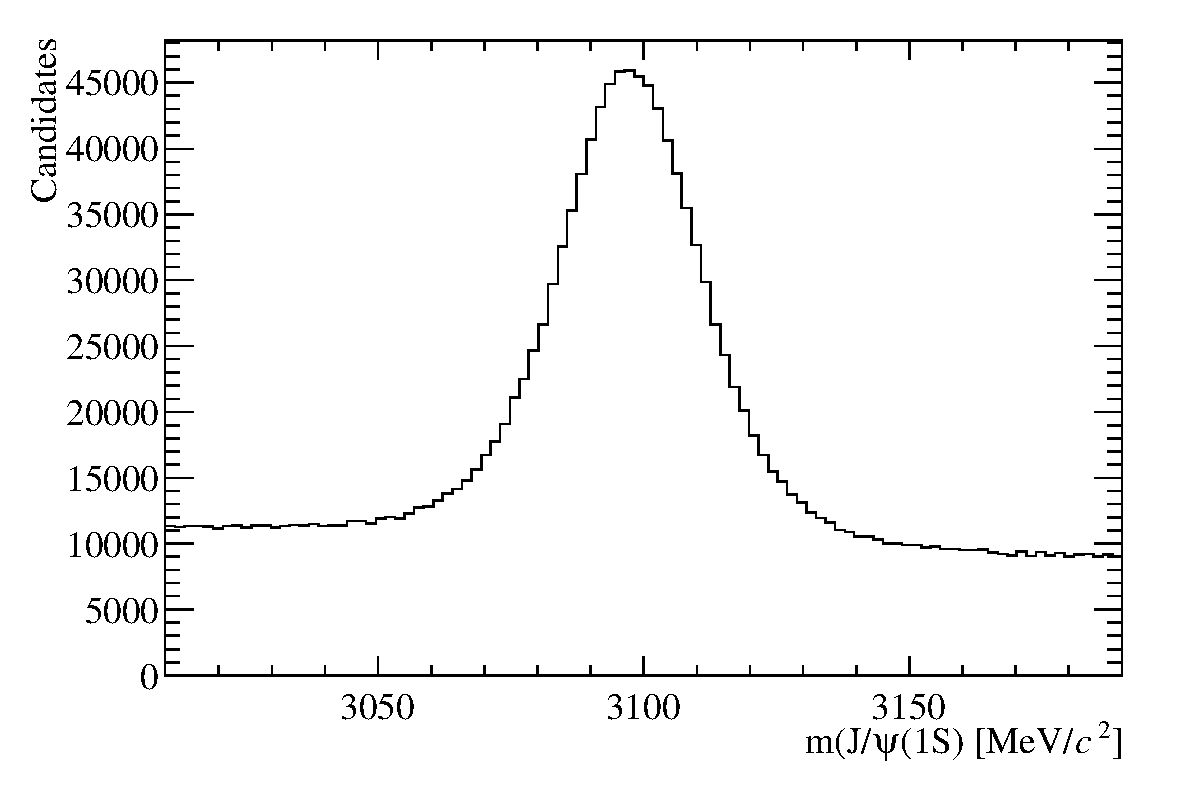
\includegraphics[width=0.75\textwidth]{figs/jpsi.pdf}\\
%\caption
{\small $\mu^+ \mu^-$ invariant mass distribution.}
%\label{fig:dmass}
\end{center}
%\end{figure}
%

Download the files jpsi.bin and jpsi-small.bin files  from the DAH Dropbox. These files contain the data recorded by LHCb in 2016 for $J/\psi \rightarrow \mu^+ \mu^-$ decays respectively. First, focus on the smalld data file (jpsi-small.bin), this contains a subset of the data. The files are written in binary format and contain seven observables for a large number of muon pairs
\begin{itemize}
\item  invariant mass of $J\psi$  candidate  in  MeV/$c^2$;
\item transverse momentum of  the dimuon candidate  candidate in MeV/$c$;
\item rapidity $\eta$ of the dimuon candidate;
\item $\chi^2$ of the geometric vertex of the dimuon candidate; 
\item Minimum transverse momentum of the two muons in MeV/$c$;
\item Minimum of a variable (ProbNNmu) that characterizes how well the two tracks forming the candidate match the hypothesis of being muons;
\item Minimum impact parameter $\chi^2$ of the two muons. The impact parameter characterizes how well the particle is matched as coming directly from a proton-proton interaction. For tracks from
 $b-$decays it should be large.
\end{itemize}

Write a python script that reads the data from this file, see below. 
\lstinputlisting{../scripts/project_F_c.py}
%\vspace*{-0.5cm}

\begin{enumerate}

\item Plot histograms of all seven variables, choosing a reasonable bin width. Always label plots correctly with title and axes and save these to a file. [Hint: The bin width should be chosen such that each of the three peaks is clearly resolved and represented by a sufficient number of bins for analysis.]

\item Next, make estimates of the peak position and width using the histogram of invariant mass.  Determine the mass from the bins with the highest number of entries in the peak regions by writing a local peak finder. By inspecting visually the muon-pair mass spectrum, determine the Full Width Half Maximum (FWHM) of the $J/\psi$ mass peak. Assuming a Gaussian signal shape estimate the mass resolution $\sigma$ from the FWHM.

\item In the  $\mu^{+}\mu^{-}$  mass spectrum define a signal region of width $\pm 30\; {\rm MeV}/c^2$ around the $J/\psi$  peak position and determine the number of events $N$ in this region. Define an upper and lower sideband region where there are only background events. These sidebands should each be half as wide as the signal region and located at masses equidistant from the $J/\psi$  peak position. Assuming that the background is falling linearly with the muon-pair mass, determine the number of background events $B$ in the signal region. Perform either a linear least squares fit in the sideband regions or use the sideband subtraction method for this. Determine the number of signal events $S$ in the signal region.

\item Construct a composite probability density
function (PDF) for the invariant mass of the muon pairs, which
contains two components : 
\begin{itemize}
\item A Gaussian shape to fit the  $J/\psi$ mass peak;
\item A shallow falling exponential to fit the background shape of the mass spectrum underneath and around the peak.
\end{itemize}

\item Use this PDF in a Maximum Likelihood fit to determine the parameters of the PDF. Note that it is essential that the composite PDF remains normalised to 1 over the range of the fit.

Determine the $J/\psi$  meson mass and yield, and all other parameters, and their and errors. Compare the measured mass with was it expected from the PDG.

You should be able to obtain the parameter errors directly from the minimization engine of your choice (scipy.optimize.minimise, scipy.optimise.curve\_fit, lmfit, see \url{https://lmfit.github.io/lmfit-py/} or Minuit). Depending on your choice you will be able to chose different minimising methods.
It would be good to show that you understand these by obtaining them yourself from the parameters of the Gaussian signal fit - this is described in the data handling lectures. Plot the fitted signal shape on top of the data. How does the fitted value of the mass compare to expectations ? 

\item The results so far probably look quite good by eye. i.e. the signal shape plotted on
top of the data probably looks like it fits quite well. However this can be misleading
when performing a precision measurement. You should make a plot of what are called
the residuals. A residual is the difference between the data in the binned histogram
and the best-fit mass model value for the centre of that bin. Describe what you see. Try repeating the exercise using the larger sample.

\item Select only events with an impact parameter $\chi^2$ larger than four and fit the data. Comment on how signal yield and the purity - ie the signal-to-background ratio change.

\item There are several ways to enhance the scope of the project. You may want to use the larger file for some of these studies.

\begin{itemize} 
\item For example, if the single
Gaussian mass model does not fit the data perfectly, one can try other mass models,
i.e. by using a signal PDF that goes beyond a single Gaussian
function. One example: is a PDF comprising a function which is the sum of two Gaussian functions (i.e. one
narrow and one wide Gaussian function to fit a single $J/\psi$ meson
peak. Alternatively try a Crystal Ball function, which incorporates a non-Gaussian tail at the lower end of
the mass peak. The functional shape is described elsewhere, e.g. see:
\begin{verbatim}
https://en.wikipedia.org/wiki/Crystal_Ball_function 
\end{verbatim} 
You could implement each of these functions in your PDF and see how much better
they are at describing the data.
\item Study how the mass and the width of the peak (the resolution)
  depends on the transverse momentum (pt) and rapidity (eta). Think about how the trends you see originate.
\item The fitted yield in bins of  pt and rapidity eta can be compared to the results for $J/\psi$ from b in the paper and with theorectical predictions. For the latter there is an online calculator that can provide you with predictions:
  \begin{verbatim}
  http://www.lpthe.jussieu.fr/~cacciari/fonll/fonllform.html
\end{verbatim} 
\item Investigate if the purity of the sample can be improved by cutting on the other variables in the file.
\end{itemize}

\end{enumerate}

\subsection{Project planning}

The project descriptions are generally significantly less detailed than what was made available for the checkpoints. Any material covered during checkpoints including python code examples are assumed to be known.  Only essential and new information is provided and you are expected to take care of the details. Python code snippets are provided where necessary, but you will have to understand yourself what they do. It is recommend that you google for information about your project on the web, including data sheets of components and python libraries, if applicable. Python scripts should be well structured, either using functions or classes.

The timeline will vary between different projects, but in general, it is recommended that you plan your work as follows:
\begin{itemize}
\item	weeks 7, 8 \& 9: 	Building your gadget and/or writing code for project;
\item	week 9, 10: 	Analysis of data or equivalent, prepare supplementary material;
\item	week 10, 11:	Finish writing of project report and prepare submission.
\end{itemize}
Note that you are advised to start writing your report as the project progresses. 

For guidance on report writing, how the projects will be assessed, plagiarism and the submission deadline, please consult the DAH course booklet and the DAH grade descriptors, available on Learn.

 


\newpage
\section{Project F4: Studies of $\chi_c$ meson properties}
%
You will use LHCb data to study the mass of P-wave $\chi_c$ mesons. The $\chi_c$ states are $c\overline{c}$ states that can decay to another $c\overline{c}$ state, the  $J/\psi$ emiting a photon. If the photon is virtual it can decay to a dimuon state. You will first make simple checks of the data and get first estimates of peak positions and widths. You will use the maximum likelihood process to fit different mass model shapes to the data. From this you will determine the parameters of the mass model for the signal peaks, and their errors. You will start with a very simple Gaussian mass model. You will then improve this and use a more sophisticated model. 

The projects have an open-ended aspect and are an opportunity where you can show your own initiative and demonstrate your experimental and computational skills.




\subsection{Detailed project description}

The $\chi_c$ states are $c\overline{c}$ states that can decay to another $c\overline{c}$ state, the  $J/\psi$ emitting a photon. If the photon is virtual it can decay to a dimuon state. 
In this project you will explore an LHCb dataset of collected $\chi_c \rightarrow J/\psi \mu^+ \mu^-$ candidates from $b$-hadron decays. The figure below shows the invariant mass distribution of selected candidates. It shows two peaks - the $\chi_{c1}$ and $\chi_{c2}$ which have spin 1 and 2 respectively.
For more information see: {DOI:10.1103/PhysRevLett.119.221801}. 
%
%\begin{figure}[htb!]
\begin{center}
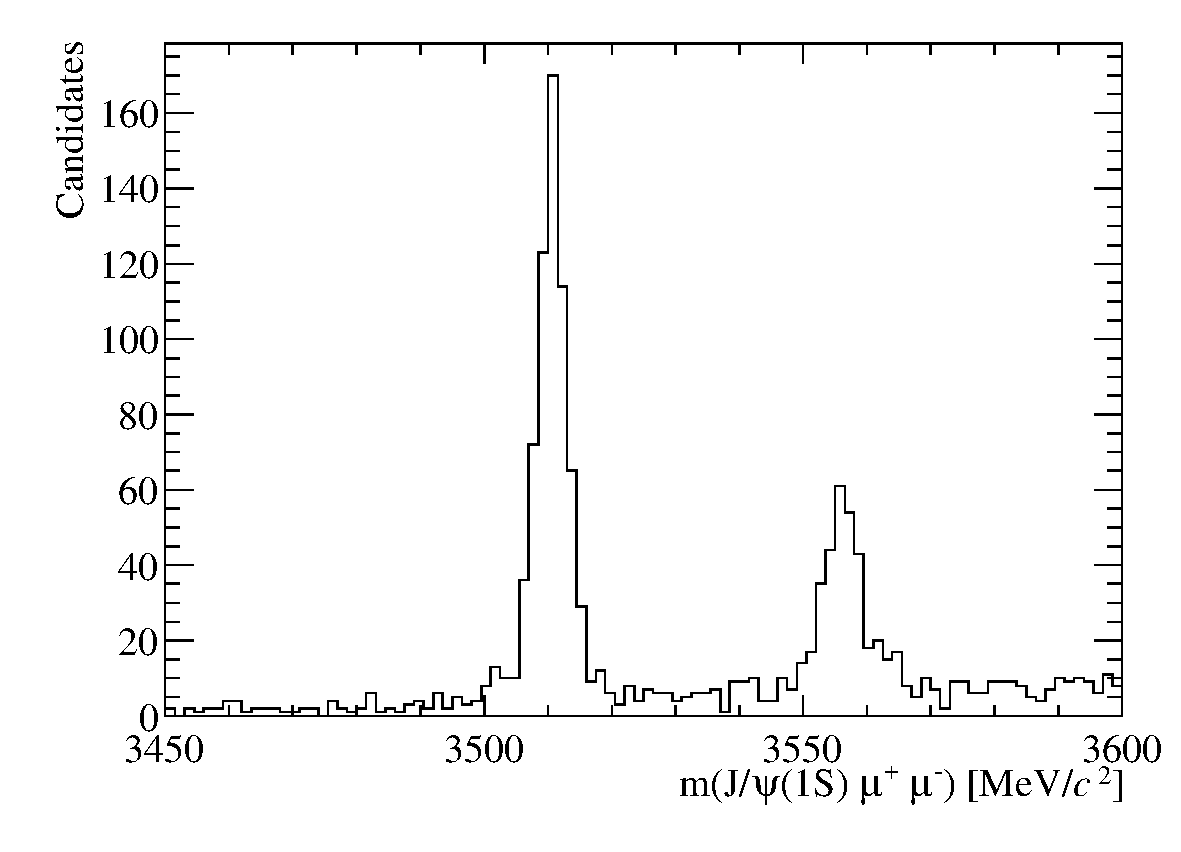
\includegraphics[width=0.75\textwidth]{figs/jmm.pdf}\\
%\caption
{\small $J/\psi \mu^+ \mu^-$ invariant mass distribution.}
%\label{fig:dmass}
\end{center}
%\end{figure}
%

Download the files chic.bin and jmm.bin files  from the DAH Dropbox, 
These files contain the data recorded by LHCb during Run 1. Focus on the chic.bin file, which selects only the invariant mass distribution around the $\chi_{c1}$ and $\chi_{c2}$ peaks. 
The files are written in binary format and contain six observables
\begin{itemize}
\item  invariant mass of $J/\psi \mu^+ \mu^-$  candidate  in  MeV/$c^2$;
\item  invariant mass of the muon pair from the virtual photon   MeV/$c^2$;
\item transverse momentum of  $J/\psi \mu^+ \mu^-$   candidate  MeV/$c$;
\item Minimum transverse momentum of the two muons in MeV/$c$;
\item Minimum of a variable (ProbNNmu) that characterizes how well the two tracks forming the candidate match the hypothesis of being muons;
\item Minimum impact parameter $\chi^2$ of the two muons. The impact parameter characterizes how well the particle is matched as coming directly from a proton-proton interaction. For tracks from
 $b-$decays it should be large.
\end{itemize}

Write a python script that reads the data from this file, see below. 
\lstinputlisting{../scripts/project_F_d.py}
%\vspace*{-0.5cm}

\begin{enumerate}

\item Plot histograms of all six variables, choosing a reasonable bin width. Always label plots correctly with title and axes and save these to a file. [Hint: The bin width should be chosen such that each of the three peaks is clearly resolved and represented by a sufficient number of bins for analysis.]

\item Next, make some estimates of the peak positions and widths using the histogram of invariant mass.  Determine the masses of the two particles by determining the bins with the highest number of entries in the peak regions. Divide the histogram into two peak regions and write a local peak finding method for this part. What is the mass differences between the $\chi_{c2}$ and $\chi_{c1}$ states ? By inspecting visually the muon-pair mass spectrum, determine the Full Width Half Maximum (FWHM) of the $\chi_{c2}$ and $\chi_{c1}$ mass peaks. Assuming a Gaussian signal shape estimate the mass resolution $\sigma$ from the FWHMs. Look up the properties of the $\chi_{c1}$ and $\chi_{c2}$ in the PDG and comment on the origin of the peak width for the two resonances.

\item In the  mass spectrum define a signal region of width $\pm 8\; {\rm MeV}/c^2$ around the $\chi_{c1}$  peak position and determine the number of events $N$ in this region. Define an upper and lower sideband region where there are only background events. These sidebands should each be half as wide as the signal region and located at masses equidistant from the $\chi_{c1}$  peak position. Assuming that the background is falling linearly with the muon-pair mass, determine the number of background events $B$ in the signal region (below the $\chi_{c1}$ peak). Perform either a linear least squares fit in the sideband regions or use the sideband subtraction method for this. Determine the number of signal events $S$ in the signal region.

\item Consider first the $\chi_{c1}$ peak which is the particle with the lowest
mass, i.e. the left most peak in the plot. Construct a composite probability density
function (PDF) for the invariant mass of the muon pairs, which
contains two components : 
\begin{itemize}
\item A Gaussian shape to fit the  $\chi_{c1}$ mass peak;
\item A shallow falling exponential to fit the background shape of the mass spectrum underneath and around the peak.
\end{itemize}

\item	Use this PDF in a Maximum Likelihood fit to determine the parameters of the PDF. Note hat it is essential that the composite PDF remains normalised to 1 over the range of the fit.

Determine the $\chi_{c1}$  meson mass and yield, and all other parameters, and their and errors.

You should be able to obtain the parameter errors directly from the minimization engine of your choice (scipy.optimize.minimise, scipy.optimise.curve\_fit, lmfit, see \url{https://lmfit.github.io/lmfit-py/} or Minuit). Depending on your choice you will be able to chose different minimising methods.
It would be good to show that you understand these by obtaining them yourself from the parameters of the Gaussian signal fit - this is described in the data handling lectures.

Plot the fitted signal shape on top of the data.

\item Now consider the entire mass range, and perform a simultaneous fit for both
peaks, and the underlying background. Again you should always report the parameter
values, and their errors. Plot the fitted signal shape on top of the data.
\item The results so far probably look quite good by eye. i.e. the signal shape plotted on
top of the data probably looks like it fits quite well. However this can be misleading
when performing a precision measurement. You should make a plot of what are called
the residuals. A residual is the difference between the data in the binned histogram
and the best-fit mass model value for the centre of that bin. Describe what you see.
\item There are several ways to enhance the scope of the project.

\begin{itemize}
\item The second file (jmm.bin) extends the $J/\psi \mu^+ \mu^-$ mass range to higher values. At higher masses more states are expected - for example radial excitations of the $\chi_c$ together with more exotic things. Plot the invariant mass distribution and with the help of the PDG try to identify the peaks you see. The other variables in the file can be used to help improve the purity of the sample and make peaks clearer. Try to fit some of the additional peaks and determine the yield and position.
\item Going to higher masses allows the production of vector mesons such as the $\phi(1020)$. This state can decay to a dimuon pair. Try selecting candidates within $\pm 10\; {\rm MeV}/c^2$ of the $\phi$ mass using the second column in the datafile. Plot the $J/\psi \mu+ \mu^-$  invariant mass distribution and with the help of the PDG try to identify the peaks you see. Again try to fit the peaks.
\item Consider replacing the Gaussian with a Voigt function. The functional shape is described elsewhere, e.g. see:
\begin{verbatim}
https://en.wikipedia.org/wiki/Voigt_profile 
\end{verbatim} 
You could implement this function in your PDF (with some help from scipy) and try to separate the contributions from the natural width and detector resolution to the line shape. Try to understand why the voigt is a better physical description of the data.

\end{itemize}



\end{enumerate}

\subsection{Project planning}

The project descriptions are generally significantly less detailed than what was made available for the checkpoints. Any material covered during checkpoints including python code examples are assumed to be known.  Only essential and new information is provided and you are expected to take care of the details. Python code snippets are provided where necessary, but you will have to understand yourself what they do. It is recommend that you google for information about your project on the web, including data sheets of components and python libraries, if applicable. Python scripts should be well structured, either using functions or classes.

The timeline will vary between different projects, but in general, it is recommended that you plan your work as follows:
\begin{itemize}
\item	weeks 7, 8 \& 9: 	Building your gadget and/or writing code for project;
\item	week 9, 10: 	Analysis of data or equivalent, prepare supplementary material;
\item	week 10, 11:	Finish writing of project report and prepare submission.
\end{itemize}
Note that you are advised to start writing your report as the project progresses. 

For guidance on report writing, how the projects will be assessed, plagiarism and the submission deadline, please consult the DAH course booklet and the DAH grade descriptors, available on Learn.

 


\newpage
\section{Project F5: Studies of $B^+ \rightarrow J/\psi K^+$}
%
You will use LHCb data to study the decay  $B^+ \rightarrow J/\psi K^+$. You will first make simple checks of the data and get first estimates of mass peak position and width. You will use the maximum likelihood process to fit different mass model shapes to the data. From this you will determine the parameters of the mass model for the signal peaks, and their errors. You will start with a very simple Gaussian mass model. You will then improve this and use a more sophisticated model. 

The projects have an open-ended aspect and are an opportunity where you can show your own initiative and demonstrate your experimental and computational skills.




\subsection{Detailed project description}
%
Large samples of the decay $B^+ \rightarrow J/\psi K^+$ have been collected by LHCb during its running. A very clean signal for this decay is observed and can be used to study a wealth of physics: $b$-hadron production, the $B^+$ lifetime and CP violation.The figure below shows the invariant mass distribution of selected candidates.
For more information see: {DOI:10.1007/JHEP12(2017)026}. 
%
%\begin{figure}[htb!]
\begin{center}
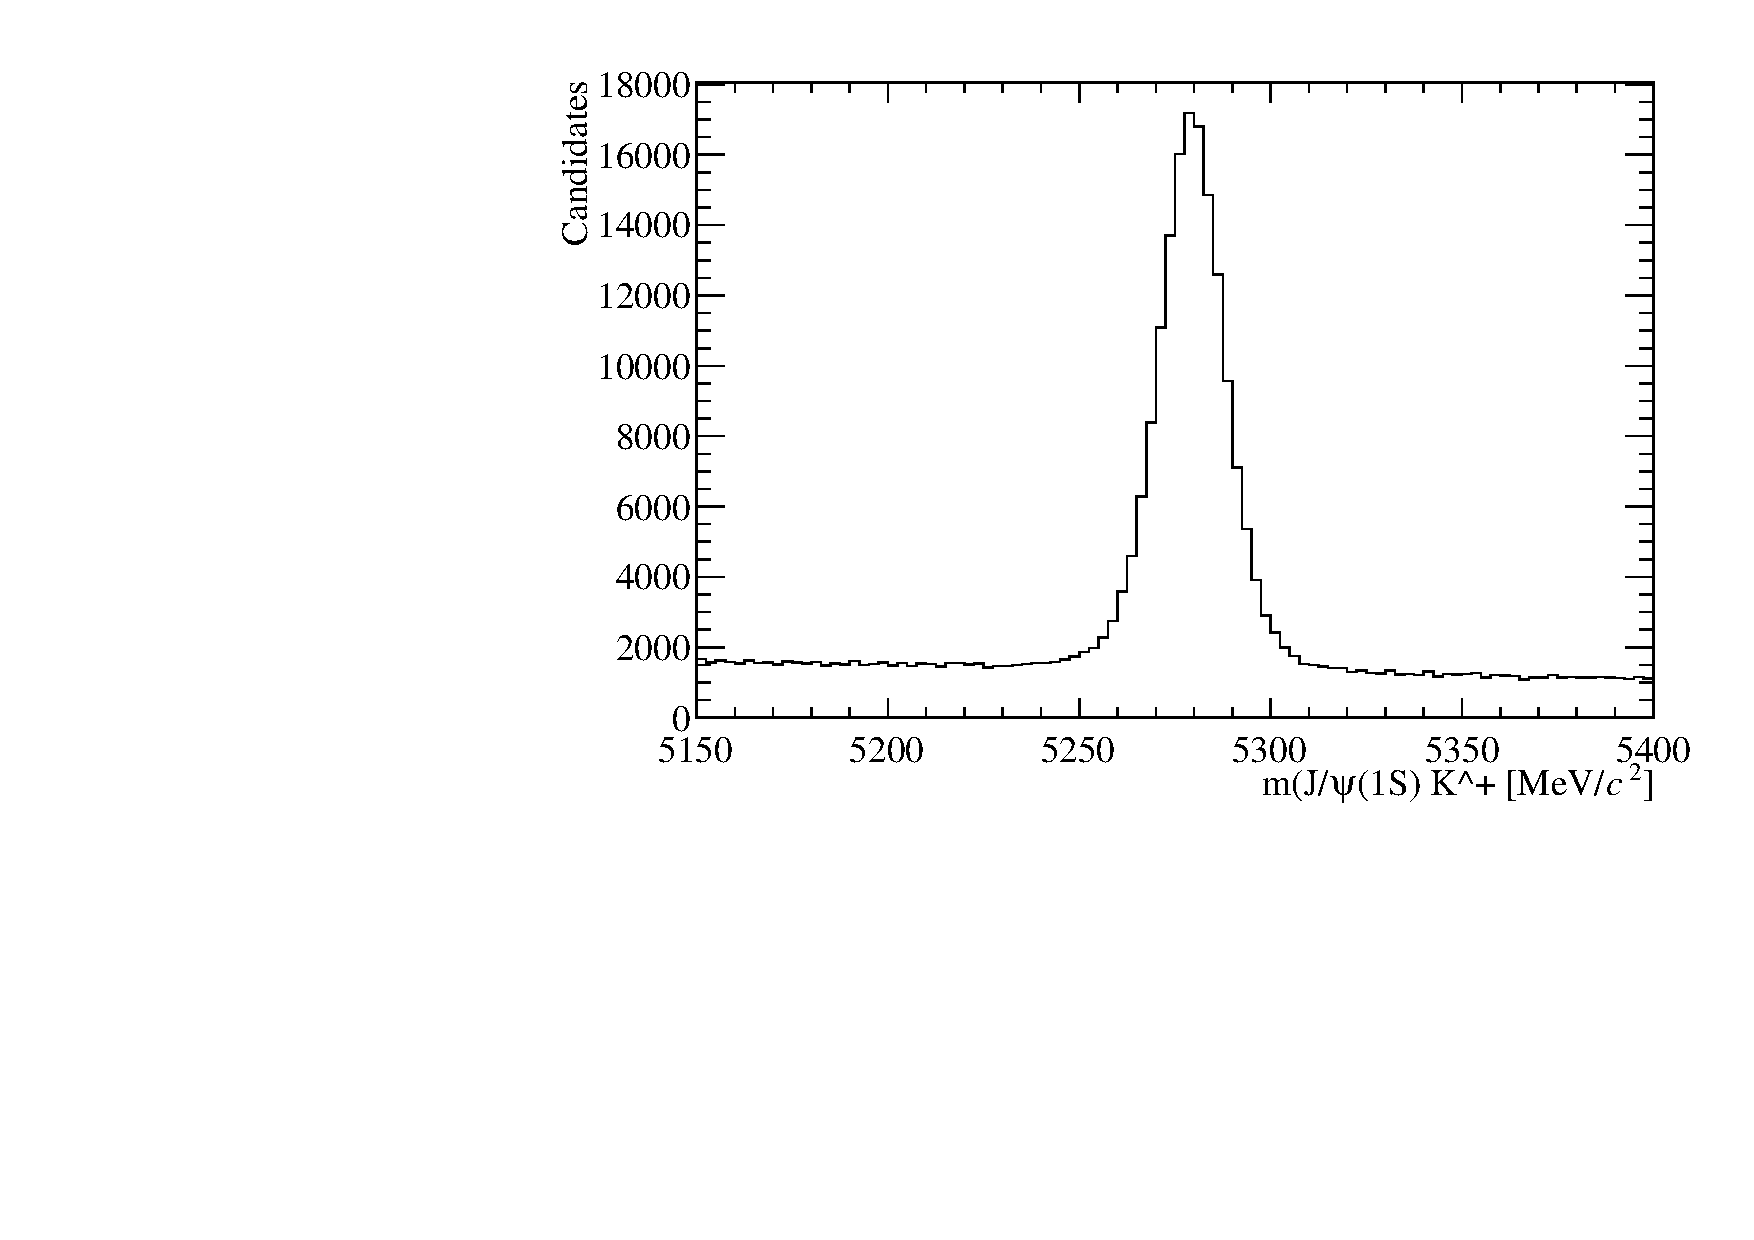
\includegraphics[width=0.75\textwidth]{figs/bmass.pdf}\\
%\caption
{\small $J/\psi K^+$ invariant mass distribution.}
%\label{fig:dmass}
\end{center}
%\end{figure}
%

Download the files kdata-small.bin and kdata.bin files  from the DAH Dropbox, 
These files contain the data recorded by LHCb during Run 1. Focus on the kdata-small.bin file,  at first which contains only a fraction of the events. 
The files are written in binary format and contain five observables
\begin{itemize}
\item  invariant mass of $J/\psi K^+$  candidate  in  MeV/$c^2$;
\item transverse momentum of  $J/\psi K^+$   candidate  MeV/$c$;
\item pseudorapidity of  $J/\psi K^+$   candidate  MeV/$c$;
\item Charge of the  candidate
\item Lifetime of the candidate in $ps$
\end{itemize}

Write a python script that reads the data from this file, see below. 
\lstinputlisting{../scripts/project_F_e.py}
%\vspace*{-0.5cm}

\begin{enumerate}

\item Plot histograms of all five variables, choosing a reasonable bin width. Always label plots correctly with title and axes and save these to a file. [Hint: The bin width should be chosen such that each of the three peaks is clearly resolved and represented by a sufficient number of bins for analysis.]

\item Next, make some estimates of the peak positions and widths using the histogram of invariant mass.  Determine the mass of the $B^+$  by determining the bins with the highest number of entries in the peak regions. Write a local peak finding method for this part. By inspecting visually the mass spectrum, determine the Full Width Half Maximum (FWHM) of the mass peak. Assuming a Gaussian signal shape estimate the mass resolution $\sigma$ from the FWHMs. How does you result for the mass compare to the PDG.

\item In the  mass spectrum define a signal region of width $\pm 25\; {\rm MeV}/c^2$ around the $B^+$  peak position and determine the number of events $N$ in this region.
  Define an upper and lower sideband region where there are only background events. These sidebands should each be half as wide as the signal region and located at masses equidistant from the peak position. Assuming that the background is falling linearly with the muon-pair mass, determine the number of background events $B$ in the signal region. Perform either a linear least squares fit in the sideband regions or use the sideband subtraction method for this. Determine the number of signal events $S$ in the signal region.

\item Construct a composite probability density
function (PDF) for the invariant mass of the muon pairs, which
contains two components : 
\begin{itemize}
\item A Gaussian shape to fit the  $B^+$ mass peak;
\item A shallow falling exponential to fit the background shape of the mass spectrum underneath and around the peak.
\end{itemize}

\item	Use this PDF in a Maximum Likelihood fit to determine the parameters of the PDF. Note hat it is essential that the composite PDF remains normalised to 1 over the range of the fit. Determine the $B^+$ meson mass and yield, and all other parameters, and their and errors.

You should be able to obtain the parameter errors directly from the minimization engine of your choice (scipy.optimize.minimise, scipy.optimise.curve\_fit, lmfit, see \url{https://lmfit.github.io/lmfit-py/} or Minuit). Depending on your choice you will be able to chose different minimising methods.
It would be good to show that you understand these by obtaining them yourself from the parameters of the Gaussian signal fit - this is described in the data handling lectures.

Plot the fitted signal shape on top of the data.

\item Now consider the entire mass range, and perform a simultaneous fit for both
peaks, and the underlying background. Again you should always report the parameter
values, and their errors. Plot the fitted signal shape on top of the data.
\item The results so far probably look quite good by eye. i.e. the signal shape plotted on
top of the data probably looks like it fits quite well. However this can be misleading
when performing a precision measurement. You should make a plot of what are called
the residuals. A residual is the difference between the data in the binned histogram
and the best-fit mass model value for the centre of that bin. Describe what you see.
\item Divide the data into $B^+$ and $B^-$ and repeat the exercise.

\item There are several ways to enhance the scope of the project. For theses studies consider to use the bigger file (kdata.bin)
  \begin{itemize}
\item If the single Gaussian mass model does not fit the data perfectly, one can try other mass models, i.e. by using a signal PDF that goes beyond a single Gaussian function.  Examples are:
\begin{itemize}
\item A PDF comprising a function which is the sum of two Gaussian functions (i.e. one narrow and one wide Gaussian function to fit the mass peak)
\item A Crystal Ball function, which incorporates a non-Gaussian tail at the lower end of the mass peak. The functional shape is described elsewhere, e.g. see: \url{http://en.wikipedia.org/wiki/Crystal_Ball_function}. 
\end{itemize}
Implement one or both of these functions in your PDF.
\item Fit the data in bins of lifetime and plot the yield in bins of time. Try to extract the lifetime of the $B^+$.
\item Perform the fit in bins of $pt$ and pseudorapidity. Compare the results to the studies of $B^+$ production in the paper and the predictions available online at
\begin{verbatim}
  http://www.lpthe.jussieu.fr/~cacciari/fonll/fonllform.html 
\end{verbatim} 

\end{itemize}
\end{enumerate}

\subsection{Project planning}

The project descriptions are generally significantly less detailed than what was made available for the checkpoints. Any material covered during checkpoints including python code examples are assumed to be known.  Only essential and new information is provided and you are expected to take care of the details. Python code snippets are provided where necessary, but you will have to understand yourself what they do. It is recommend that you google for information about your project on the web, including data sheets of components and python libraries, if applicable. Python scripts should be well structured, either using functions or classes.

The timeline will vary between different projects, but in general, it is recommended that you plan your work as follows:
\begin{itemize}
\item	weeks 7, 8 \& 9: 	Building your gadget and/or writing code for project;
\item	week 9, 10: 	Analysis of data or equivalent, prepare supplementary material;
\item	week 10, 11:	Finish writing of project report and prepare submission.
\end{itemize}
Note that you are advised to start writing your report as the project progresses. 

For guidance on report writing, how the projects will be assessed, plagiarism and the submission deadline, please consult the DAH course booklet and the DAH grade descriptors, available on Learn.

 




\begin{comment}
\newpage
\section{Project F3old: Make Accurate Measurements of Particle Masses}

\subsection{Goals of project}

You will use LHCb data on the invariant mass of particle candidates that you were introduced to during a checkpoint. You will analyse this in a much more sophisticated way and closer to the actual analysis performed leading to its publication. You will use the maximum likelihood process to fit different mass model shapes to the data. From this you will determine the parameters of the mass model for the three signal peaks, and their errors. You will start with a very simple Gaussian mass model. You will then improve this and use a more sophisticated model.

The projects have an open-ended aspect and are an opportunity where you can show your own initiative and demonstrate your experimental and computational skills. 



\subsection{Detailed project description}

You were previously introduced to the LHCb Upsilon data. In this
project you will explore another LHCb dataset where a $\psi(2S)$ meson
(a bound $c\overline{c}$ state) and a pair of
oppositely pions have been combined. Two clear
peaks are observed in this mass spectrum corresponding to the $B_s$
and $B^0$ mesons, see figure below %(Fig.~\ref{fig:bmass}). 
The background shape is quite
complex. At higher masses it is exponential in shape. At lower masses
there is an additional background from the decay $B^0 \rightarrow
\psi(2S) K^+ \pi^-$ where the kaon has been incorrectly identified as
a pion. For more information see: {DOI: 10.1016/j.nuclphysb.2013.03.004 and DOI: 10.1016/j.physletb.2015.06.038}.


During checkpoint 6, you performed some very simple "peak finding". In this project you are going to do the analysis much like it would actually be carried out in a particle physics experiment.

%
%\begin{figure}[htb!]
\begin{center}
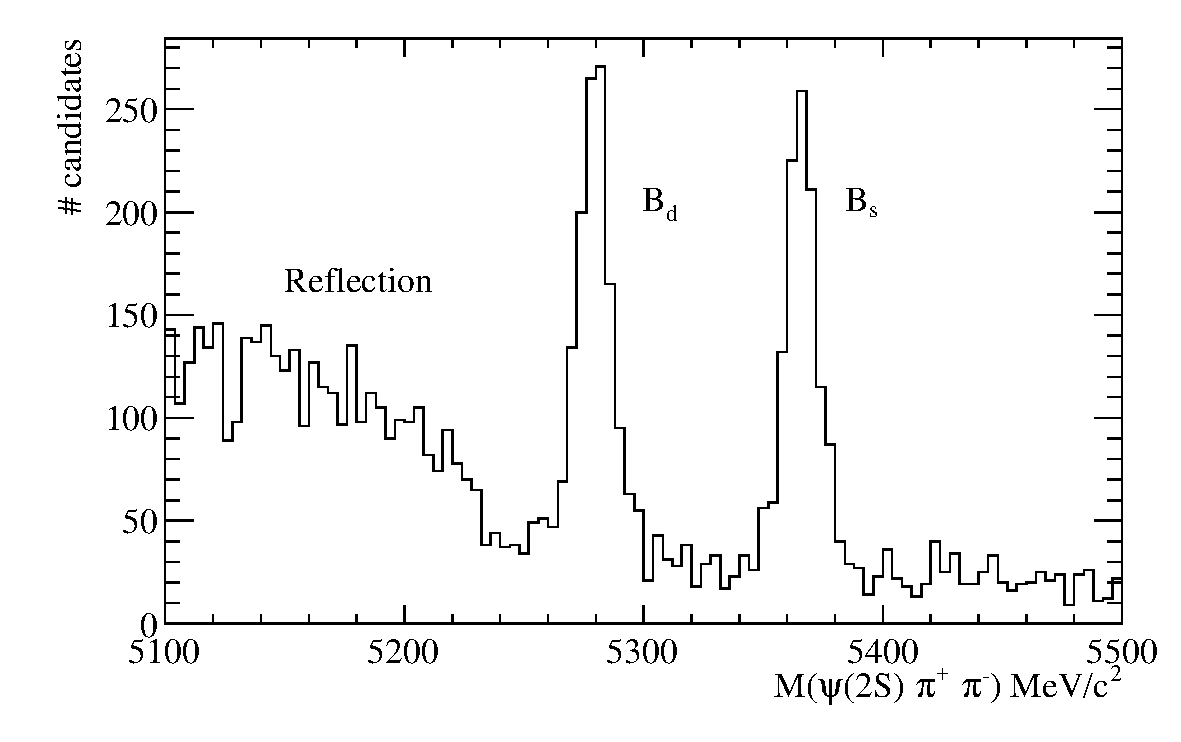
\includegraphics[width=0.75\textwidth]{figs/psi2Spipi.pdf}\\
%\caption
{\small $\psi ({\rm 2S}) \pi^{+} \pi^{-}$  invariant mass distribution.}
%\label{fig:bmass}
\end{center}
%\end{figure}
%


\begin{enumerate}


\item Consider first the $B_s$ peak which is the particle with the highest
mass, i.e. the right most peak in the plot. Construct a composite probability density
function (PDF) for the invariant mass of the muon pairs, which
contains two components :

\begin{itemize}
\item A Gaussian shape to fit the $B_s$ peak;
\item A shallow falling exponential to fit the background shape of the mass spectrum
underneath the peak.
\end{itemize}

\item Use this PDF in a Maximum Likelihood fit to determine the parameters of the PDF.
Note hat it is essential that the composite PDF remains normalised to 1 over the range
of the fit. 

Determine the $B_s$ meson mass and yield, and all other parameters, and their and
errors.

You should be able to obtain the parameter errors directly from the minimization engine of your choice (scipy.optimize.minimise, scipy.optimise.curve\_fit, lmfit, see \url{https://lmfit.github.io/lmfit-py/} or Minuit). Depending on your choice you will be able to chose different minimising methods.
It would be good to show that you understand these by obtaining them yourself from the parameters of the Gaussian signal fit - this is described in the data handling lectures.

Plot the fitted signal shape on top of the data.

\item Now consider the mass range above the reflection, and perform a simultaneous fit for both
peaks, and the underlying background. Again you should always report the parameter
values, and their errors. Plot the fitted signal shape on top of the data.

\item The results so far probably look "quite good" by eye.  i.e. the signal shape plotted on top of the data probably looks like it fits quite well.  However this can be misleading when performing a precision measurement.  You should make a plot of what are called the "residuals". A residual is the difference between the data in the binned histogram and the best-fit mass model value for the centre of that bin. Describe what you see.

\newpage

\item There are several ways to enhance the scope of the project.

\begin{itemize} 
\item For example, if the single
Gaussian mass model does not fit the data perfectly, one can try other mass models,
i.e. by using a signal PDF that goes beyond a single Gaussian
function. One example: is a PDF comprising a function which is the sum of two Gaussian functions (i.e. one
narrow and one wide Gaussian function to fit a single D meson
peak. Alternatively try a Crystal Ball function, which incorporates a non-Gaussian tail at the lower end of
the mass peak. The functional shape is described elsewhere, e.g. see:
\begin{verbatim}
https://en.wikipedia.org/wiki/Crystal_Ball_function 
\end{verbatim} 
You could implement each of these functions in your PDF and see how much better
they are at describing the data.
\item Try to extend the fit to include the kinematic reflection
\item Read the publication and see what is said about systematic errors. Make a reasonable
attempt at determining some systematic errors on the masses.
\item Compare your results to the PDG and previous measurements.
\item From the yields of $B_s$ and $B^0$ mesons, following the
  procedures in the papers try to evaluate the ratio of branching
  ratios of these modes.
\end{itemize}


\end{enumerate}

\subsection{Project planning}

The project descriptions are generally significantly less detailed than what was made available for the checkpoints. Any material covered during checkpoints including python code examples are assumed to be known.  Only essential and new information is provided and you are expected to take care of the details. Python code snippets are provided where necessary, but you will have to understand yourself what they do. It is recommend that you google for information about your project on the web, including data sheets of components and python libraries, if applicable. Python scripts should be well structured, either using functions or classes.

The timeline will vary between different projects, but in general, it is recommended that you plan your work as follows:
\begin{itemize}
\item	weeks 7, 8 \& 9: 	Building your gadget and/or writing code for project;
\item	week 9, 10: 	Analysis of data or equivalent, prepare supplementary material;
\item	week 10, 11:	Finish writing of project report and prepare submission.
\end{itemize}
Note that you are advised to start writing your report as the project progresses. 

For guidance on report writing, how the projects will be assessed, plagiarism and the submission deadline, please consult the DAH course booklet and the DAH grade descriptors, available on Learn.

 
\end{comment}

